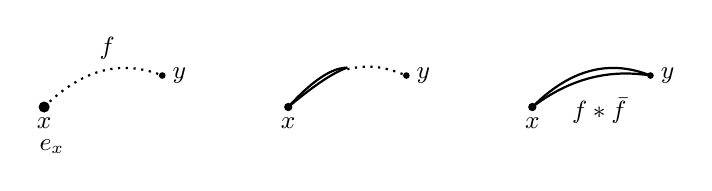
\begin{tikzpicture}[line width=0.8pt, every node/.style={font=\small}]
  % t = 0: constant path at x (f dotted for reference)
  \draw[dotted] (0,0) .. controls (0.5,0.5) and (1.0,0.6) .. (1.5,0.4);
  \fill (0,0) circle (2pt) node[below] {$x$};
  \fill (1.5,0.4) circle (1.2pt) node[right] {$y$};
  \node at (0.8,0.75) {$f$};
  \node at (0.1,-0.5) {$e_x$};
  \node at (2.4,0.2) {$\rightsquigarrow$};
  % intermediate t: go out along f to f(t) and come back
  \begin{scope}[shift={(3.1,0)}]
    \draw[dotted] (0.75,0.48) .. controls (1.05,0.55) and (1.25,0.5) .. (1.5,0.4);
    \fill (1.5,0.4) circle (1.2pt) node[right] {$y$};
    \draw (0,0) .. controls (0.3,0.33) and (0.55,0.5) .. (0.75,0.5);
    \draw (0,0) .. controls (0.3,0.25) and (0.55,0.43) .. (0.75,0.5);
    \fill (0,0) circle (1.5pt) node[below] {$x$};
  \end{scope}
  \node at (5.5,0.2) {$\rightsquigarrow$};
  % t = 1: f * fbar
  \begin{scope}[shift={(6.2,0)}]
    \draw (0,0) .. controls (0.5,0.5) and (1.0,0.6) .. (1.5,0.4);
    \draw (0,0) .. controls (0.5,0.38) and (1.0,0.48) .. (1.5,0.4);
    \fill (0,0) circle (1.5pt) node[below] {$x$};
    \fill (1.5,0.4) circle (1.2pt) node[right] {$y$};
    \node at (0.85,-0.05) {$f*\bar f$};
  \end{scope}
\end{tikzpicture}
